\documentclass[12pt,a4paper,oneside,openany]{book}

\usepackage[utf8]{inputenc}
\usepackage{tikz}
\usepackage{minted}
\graphicspath{{img/}}


%% Change these:
\newcommand{\projecttitle}{Pibot: - Worlds first paraplegic robot}
\newcommand{\projectauthor}{Aaron Flanagan \\[0.2cm] Ciaran Brennan \\[0.2cm] David Hynes}
\newcommand{\projectadvisor}{Damien Costello}
\newcommand{\projectprogramme}{B.Sc.(Hons) in Software Development}
\newcommand{\projectdate}{\today}
%% End of things to change.

\begin{document}
\begin{titlepage}
	\begin{center}
		
\includegraphics{gmit-logo.jpg}
	\end{center}
	\begin{minipage}[t][6cm]{\textwidth}
		\centering
		\rule{\linewidth}{0.5mm} \\[0.4cm]
		{ \LARGE \bfseries \projecttitle \\[0.4cm] }
		\rule{\linewidth}{0.5mm} \\[0.8cm]
	\end{minipage}
	
	\begin{minipage}[t][6.5cm]{\textwidth}
		\centering
		\textbf{\projectauthor}\\[0.5cm]
		\projectprogramme
	\end{minipage}
	
	\begin{minipage}[t][1cm]{\textwidth}
		\centering
		\textsc{\projectdate}
	\end{minipage}
	
	\begin{minipage}[t][3cm]{\textwidth}
		\centering
		\textbf{Gesture Based UI Project}\\[0.3cm]
		Advised by: \projectadvisor \\[0.1cm]
		Department of Computer Science and Applied Physics\\
		Galway-Mayo Institute of Technology (GMIT)
	\end{minipage}
\end{titlepage}

\chapter*{About this project}

\paragraph{Abstract}
This project suggests the idea of a human controlled search and rescue robot. Most of the current search and rescue robots available are remote control and require some knowledge and training to control. What if anyone in the blink of an eye can resume control over this device and potentially save lives in process.

\chapter*{Purpose of the application}
Our project plan is to use a Raspberry PI to pick up and display the pose types of the users hand from the Myo device. We have set it up so that when we move our arm in a specific direction or a specific way, LED lights on a circuit board will light up corresponding to the movement used. This is to simulate movement on our robot because the necessary parts for the motors were unavailable to use. This project can easily be expanded if we had access to hardware for it. Our primary example of expansion was to put wheels on the Raspberry PI instead of LED lights. It would have the same concept but instead the wheels would turn according to our Myo arm movement. The range of Raspberry PI hardware is vast and creative things can be done with the Myo and the Raspberry PI once the core basics are grasped, and that is our aim for this project.
Our original plan was a robot with wheels and camera that can be used for search and rescue missions and for going to places we dare not go ourselves, like a burning building. This is just a concept and solving world economic crisis with our trained Raspberry Pi bots comes later.

\chapter*{Gestures identified}
Gestures that would be appropriate for this application would be anything from thrusting arm to clenching fist depending on the hardware we attach to the Raspberry PI. For example, if we had wheels attached, we could do a thrusting motion with our fist to accelerate the wheels. The acceleration speed would depend how fast we move our fist. Stopping the wheel movement could be done by making a ‘stop’ sign with our fist.

\includegraphics{stop.jpg}
To turn, we could move our hand to the left or right, which could also be combined with other gestures to break or accelerate at the same time as turning the wheels. The possibilities are vast.
The idea was a motion controlled robot over the most commonly used remote controlled robot. Anyone can put this band on and assume control at a given moment.
Another example of how we could incorporate gestures into our idea is a zoom and screenshot function for our camera. For our zoom in/out method we could make a circle with our fingers and extend or retract our fingers to zoom in or out. This would take some research to complete as there would be issues with zooming along with controlling the wheels. The screenshot function could be done by double clenching our fist and having a default save location on the Raspberry pie to which all the screenshots are saved automatically. 


\chapter*{Architecture \& Hardware}
The hardware we used for this project is as follows:

\begin{itemize}
	\item PI CameraPI Camera 
	\item LED lights
	\item Breadboard
	\item Raspberry Pi
	\item Male/Female connection cables
	\item Resistors.
	\item External network adapter
	\item Myo motion sensor device
\end{itemize}

The main component is the Raspberry PI. An external network adapter is used to connect to a network for internet access. The camera is used to stream what the robot sees back to the screen. The raspberry pi isn’t a very powerful device the the frame rate is quite slow. 
It uses the connection cables to connect the breadboard to the pin headers on the Raspberry PI.  220 kb resistors are then used to wire the LEDs to a ground current. They are then programmed to flash to simulate motor movement using python and the GPIO library available. Finally we use the myo armband to control the robots movement. If a fist pose is made the robot moves forward, if a stop pose is made it stops. If the hand is left or right it turns. A problem occurred that the Myo wouldn’t connect to the Raspberry PI. Myo doesn’t have Linux support so we had to find a custom made package. PyoConnect (INSERT LINK) was used, it is a python made library that reflects the original LUA library. It can be found at www.fernandocosentino.net/pyoconnect/. The operating system we use is Raspbian which is a Debian based system and this library is made for Debian operating systems however it wouldn’t connect. It did connect to an Ubuntu system on one of the developers laptops so we wrote the script on this to show how it would of worked if there wasn’t a hardware compatibility issue.

\begin{figure}[!b]
	\begin{minipage}[b]{0.47\textwidth}
		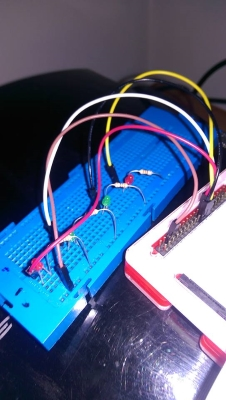
\includegraphics{raspberry.jpg}
		\caption{Raspberry Pi and breadboard all connect together.}
	\end{minipage}
	\hfill
	\begin{minipage}[b]{0.47\textwidth}
		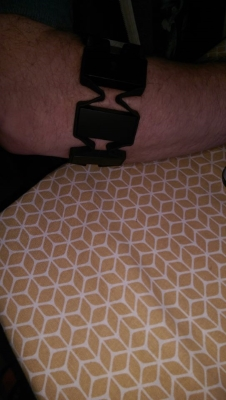
\includegraphics{myo.jpg}
		\caption{Myo armband being used. Bluetooth connection to the PI.}
	\end{minipage}
\end{figure}

\chapter*{Conclusions and Recommendations}
We have learned that the Myo and Raspberry PI are not naturally compatible due to the fact Linux is not supported by the Myo to work with. In future we would either have to do more research on adapting code to make the compatibility issues non-existent or we would try and find a windows mini-computer, which would probably be the better of the two ideas until more support for Linux is enabled for the Myo. Next time we would advise possibly changing it to an Internet of Things project to avoid platform dependent problems. The use of an Arduino board might be a better decision for the LEDS because the raspberry pi is timely on start-up and connecting the internet. Also a Kinect sensor to read human movements might be worth a try because the Myo has to be “warmed” up to be used and in an emergency this isn’t acceptable.

\chapter*{Code}

Camera.py
\begin{minted}{python}
# import the necessary packages
from picamera.array import PiRGBArray
from picamera import PiCamera
import time
import cv2

class Camera(object):
def runCam():
# initialize the camera and grab a reference to the raw camera capture
 camera = PiCamera()
 camera.resolution = (640, 480)
 camera.vflip = True
 camera.framerate = 72
 rawCapture = PiRGBArray(camera, size=(640, 480))

 camera.start_preview()

 time.sleep(0.1)

 # capture frames from the camera
 for frame in camera.capture_continuous(rawCapture, format="bgr",
  use_video_port=True):
 # grab the raw NumPy array representing the image, then initialize the timestamp
 # and occupied/unoccupied text
 image = frame.array

 # show the frame
 cv2.imshow("Frame", image)
 key = cv2.waitKey(1) & 0xFF

 # clear the stream in preparation for the next frame
 rawCapture.truncate(0)

 # if the `q` key was pressed, break from the loop
 if key == ord("q"):
 break
\end{minted}

\pagebreak
Pibot.py
\begin{minted}{python}
import RPi.GPIO as GPIO
import time

eight = 8
seven = 7
nine = 9
eleven = 11

GPIO.setmode(GPIO.BCM)
GPIO.setup(eight,GPIO.OUT)
GPIO.setup(seven,GPIO.OUT)
GPIO.setup(nine,GPIO.OUT)
GPIO.setup(eleven,GPIO.OUT)

class Bot(object):

def right(self):
 i = 0
 while i < 2:
 GPIO.output(eight,GPIO.HIGH)
 time.sleep(.9)
 GPIO.output(eight,GPIO.LOW)
 time.sleep(.5)
 i = i + 1

def left(self):
 i = 0
 while i < 2:
 GPIO.output(seven,GPIO.HIGH)
 time.sleep(.9)
 GPIO.output(seven,GPIO.LOW)
 time.sleep(.5)
 i = i + 1

def forward(self):
 i = 0
 while i < 2:
 GPIO.output(nine,GPIO.HIGH)
 time.sleep(.9)
 GPIO.output(nine,GPIO.LOW)
 time.sleep(.5)
 i = i + 1

def back(self):
 i = 0
 while i < 2:
 GPIO.output(eleven,GPIO.HIGH)
 time.sleep(.9)
 GPIO.output(eleven,GPIO.LOW)
 time.sleep(.5)
 i = i + 1

 #Bot().left()
 #Bot().right()
 #Bot().back()
 #Bot().forward()
\end{minted}

\pagebreak
controller.py
\begin{minted}{python}
import sys
import time
sys.path.append('lib/')

from myo import Myo
from camera import Camera
from pibot import Bot
from print_pose_listener import PrintPoseListener
from vibration_type import VibrationType

def main():
 print('Start Myo for Linux')

 listener = PrintPoseListener()
 myo = Myo()

 try:
  myo.connect()
  myo.add_listener(listener)
  myo.vibrate(VibrationType.SHORT)
  while True:
   myo.run()
   print(listener.getPose())
   time.sleep(2)


 except KeyboardInterrupt:
  pass
 except ValueError as ex:
  print(ex)
 finally:
  myo.safely_disconnect()
  print('Finished.')

if __name__ == '__main__':
main()

\end{minted}

\pagebreak
pyoconnect.py
\begin{minted}{python}
#from pibot import Bot
#from camera import Camera

def onPoseEdge(pose, edge):
 print("OnPoseEDGE: " + pose)

 #camera.runCam()

 if (pose == "waveOut"):
  #Bot.right()

 if (pose == "waveIn"):
  #Bot.left()		

 if (pose == "fist"):
  #Bot.left()	
  #Bot.right()

 if(pose == "fingerSpread"):
  #Bot.stop()	
\end{minted}

\end{document}          
